% Asset ID: FA21ConicSections2EnrichmentTikZ-005
% Source: hyperbola tangent intercept locus evidence
% Boundary status: Off-spec enrichment until official CCEA conics evidence is supplied.
\documentclass[tikz,border=8pt]{standalone}
\usepackage{amsmath,amssymb}
\usetikzlibrary{arrows.meta,calc,positioning}
\definecolor{Canvas}{HTML}{FAF9F6}
\definecolor{Ink}{HTML}{2C2C2E}
\definecolor{Gold}{HTML}{C5A059}
\definecolor{GoldDeep}{HTML}{D4AF37}
\begin{document}
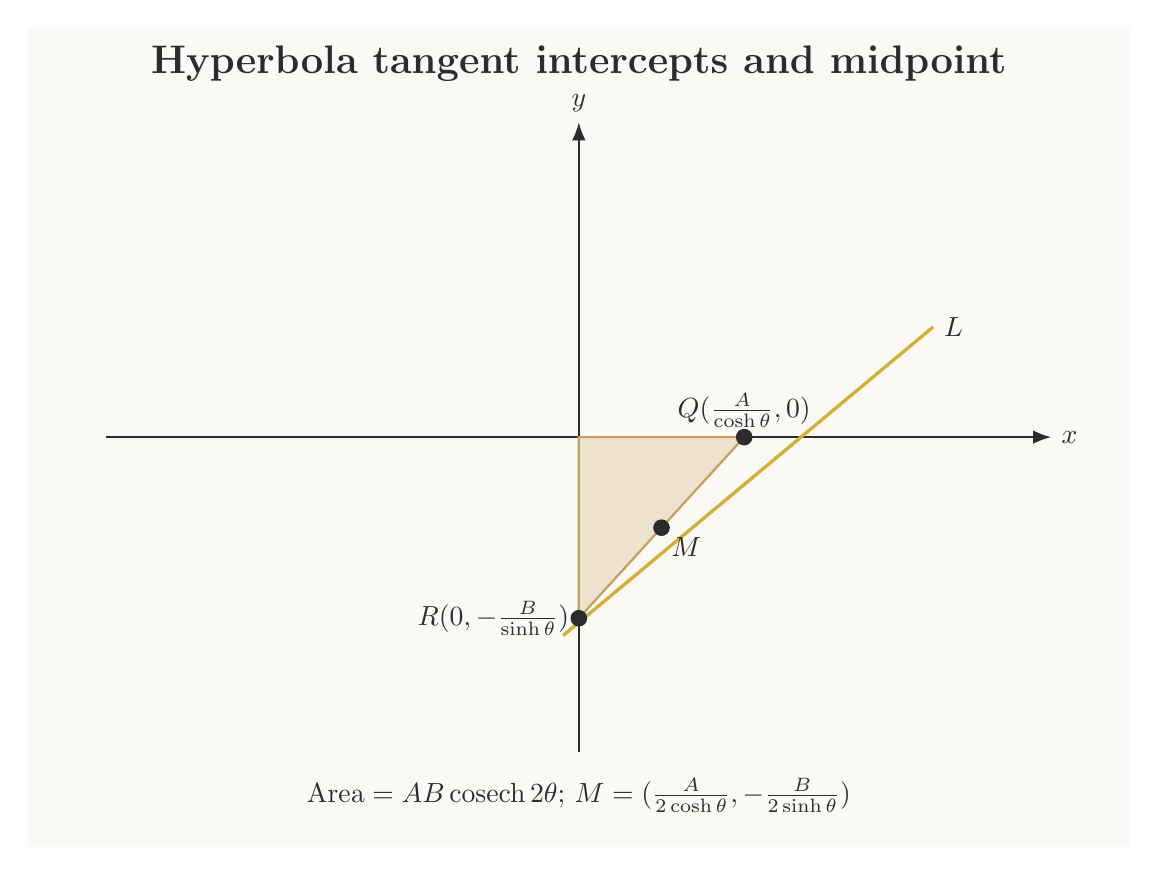
\begin{tikzpicture}[x=1cm,y=1cm,>=Latex]
\fill[Canvas] (-7,-5.2) rectangle (7,5.2);
\node[Ink, font=\Large\bfseries] at (0,4.75) {Hyperbola tangent intercepts and midpoint};
\draw[Ink, thick, -Latex] (-6,0)--(6,0) node[right] {$x$};\draw[Ink, thick, -Latex] (0,-4)--(0,4) node[above] {$y$};\coordinate (Q) at (2.1,0);\coordinate (R) at (0,-2.3);\coordinate (M) at (1.05,-1.15);\draw[GoldDeep, very thick] (-.2,-2.52)--(4.5,1.4) node[right,Ink] {$L$};\fill[Gold, opacity=.25] (0,0)--(Q)--(R)--cycle;\draw[Gold, thick] (0,0)--(Q)--(R)--cycle;\fill[Ink] (Q) circle (3pt) node[above] {$Q(\frac{A}{\cosh\theta},0)$};\fill[Ink] (R) circle (3pt) node[left] {$R(0,-\frac{B}{\sinh\theta})$};\fill[Ink] (M) circle (3pt) node[below right] {$M$};\node[Ink, align=left] at (0,-4.55) {$\text{Area}=AB\operatorname{cosech}2\theta$; $M=(\frac{A}{2\cosh\theta},-\frac{B}{2\sinh\theta})$};
\end{tikzpicture}
\end{document}
